\chapter{Multichannel azimuth reconstruction and topography}\label{ch:recon}

\section{Aliased channels and folded parcels}

Each channel is sampled at $\PRFop=\PRF/\Nrx$, below $\Ba=\SI{1235}{Hz}$, so every channel frequency
$\phi\in[-\PRFop/2,\PRFop/2)$ is the sum of $\Nrx$ \emph{parcels} of the full-rate spectrum $U$ at
\begin{equation}
  f_q = \phi + q\,\PRFop - \tfrac{\Nrx-1}{2}\PRFop, \qquad q=0,\dots,\Nrx-1 ,
\end{equation}
each weighted by the channel transfer function $H_i$:
\begin{equation}
  S_i(\phi) = \sum_{q} H_i(f_q)\, U(f_q)
  \quad\Longleftrightarrow\quad
  \bm{s}(\phi) = \mathbf{H}(\phi)\,\bm{u}(\phi),
  \label{eq:fold}
\end{equation}
with $\bm{s}$ the $\Nrx$ channel spectra and $\bm{u}$ the $\Nrx$ parcels. The standard reconstruction
\cite{Krieger2004,Gebert2009} inverts this system at every $\phi$, $\hat{\bm u}=\mathbf H^{-1}\bm s$ with
$H_{iq}(\phi)=H_i(f_q)$ from \eqref{eq:Hi} for the reference point, and puts each parcel back at its frequency.

Doppler frequency $f$ seen from azimuth $x_c$ maps to the ground position
\begin{equation}
  x(f) = x_c + r_0 \tan\!\bigl(\arcsin(\lambda f/2v)\bigr) \approx x_c + \frac{\lambda r_0}{2v}\, f ,
  \label{eq:ruler}
\end{equation}
(the \emph{ruler}), so parcels one $\PRFop$ apart come from positions
\begin{equation}
  X \approx \frac{\lambda r_0\,\PRFop}{2v} \qquad (\SI{6.23}{km}\text{ for } \PRFop=\SI{500}{Hz}),
\end{equation}
apart (\SI{0.81}{s}): one bin of an aliased channel mixes the terrain at $x$, $x\pm X$, $x\pm 2X,\dots$
(\cref{fig:folding}).

\begin{figure}[htbp]
\centering
\begin{tikzpicture}[>=Latex,xscale=1.3,yscale=0.85]
  % full-rate band: PRF = 8 units, PRF_op = 2 units, Ba = 4.94 units (1235 Hz of 2000 Hz)
  \draw[->] (-4.4,0) -- (4.7,0) node[right,font=\small]{$f$ (full rate)};
  \fill[cocc!15] plot[smooth,domain=-2.47:2.47,samples=41] (\x,{2.2*cos(\x*90/2.47)^2}) -- cycle;
  \draw[cocc,thick] plot[smooth,domain=-2.47:2.47,samples=41] (\x,{2.2*cos(\x*90/2.47)^2});
  \foreach \b in {-4,-2,0,2,4} \draw[gray,dashed] (\b,-0.1) -- (\b,2.55);
  \foreach \q/\c in {0/-3,1/-1,2/1,3/3} \node[font=\scriptsize] at (\c,2.75) {parcel $q=\q$};
  \draw[<->] (2,-0.4) -- node[below,font=\scriptsize]{$\PRFop$} (4,-0.4);
  \draw[<->] (-2.47,3.25) -- node[above,font=\scriptsize]{$\Ba$} (2.47,3.25);
  \draw[<->] (-4,3.95) -- node[above,font=\scriptsize]{$\PRF=\Nrx\,\PRFop$} (4,3.95);
  % the same channel bin phi in every parcel
  \foreach \f in {-2.25,-0.25,1.75} {\draw[cnone,thick] (\f,0) -- (\f,{2.2*cos(\f*90/2.47)^2}); \fill[cnone] (\f,0) circle (0.05);}
  \fill[gray] (3.75,0) circle (0.05);
  % channel axis
  \draw[->] (-1.2,-2.6) -- (1.4,-2.6) node[right,font=\small]{$\phi$ (channel $i$, rate $\PRFop$)};
  \draw[gray,dashed] (-1,-2.7) -- (-1,-2.2); \draw[gray,dashed] (1,-2.7) -- (1,-2.2);
  \fill[cnone] (0.75,-2.6) circle (0.06);
  \foreach \f in {-2.25,-0.25,1.75} \draw[->,cnone!70] (\f,-0.08) to[out=-90,in=100] (0.73,-2.5);
  \node[font=\scriptsize,anchor=west,align=left] at (2.3,-1.75) {one bin of channel $i$:\\ $S_i(\phi)=\sum_q H_i(f_q)\,U(f_q)$};
  % ground positions through the ruler
  \begin{scope}[yshift=-4.6cm]
    \fill[terrainfill] (-4.3,-0.25) -- plot[smooth] coordinates {(-4.3,0.1) (-3.2,0.5) (-2.1,0.25) (-1.0,0.95) (-0.1,0.45) (1.0,0.2) (1.9,1.05) (3.0,0.4) (3.9,0.7) (4.6,0.3)} -- (4.6,-0.25) -- cycle;
    \draw[terrain,thick] plot[smooth] coordinates {(-4.3,0.1) (-3.2,0.5) (-2.1,0.25) (-1.0,0.95) (-0.1,0.45) (1.0,0.2) (1.9,1.05) (3.0,0.4) (3.9,0.7) (4.6,0.3)};
    \foreach \xx/\lab in {-2.25/{x-X},-0.25/{x},1.75/{x+X}} {\fill[cnone] (\xx,-0.25) circle (0.06); \node[font=\scriptsize,below] at (\xx,-0.3) {$\lab$};}
    \fill[gray] (3.75,-0.25) circle (0.06); \node[font=\scriptsize,below,gray] at (3.75,-0.3) {$x+2X$ (outside $\Ba$)};
    \node[font=\scriptsize,anchor=east] at (-4.35,0.1) {terrain $h(x)$};
  \end{scope}
\end{tikzpicture}
\caption[Folding of the Doppler spectrum]{Folding in an aliased channel ($\Nrx=4$): the parcels of one bin come, through
\eqref{eq:ruler}, from ground positions $X$ apart, in general at different heights.}
\label{fig:folding}
\end{figure}

On flat terrain the standard reconstruction recovers the full-rate spectrum (\cref{fig:spectra}).

\begin{figure}[htbp]
\centering
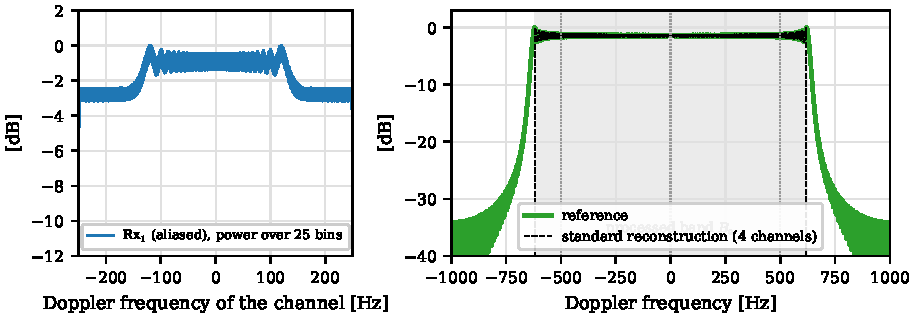
\includegraphics[width=\linewidth]{figures/spectra_reconstruction.pdf}
\caption[Aliased channel and reconstructed spectrum]{One target at $h=0$, default formation. Left: one channel at
\SI{500}{Hz} (averaged over 25 bins), parcels overlapping. Right: reference and standard reconstruction at the full PRF; grey:
$\Ba$; dotted: parcel borders, $\PRFop$ apart.}
\label{fig:spectra}
\end{figure}

\section{How topography creates ambiguities}\label{sec:mismatch}

A scatterer at height $h$ adds the phase $\e^{-\jj\varphi_i}$ of \eqref{eq:dc0}: $\bm s=\mathbf D\mathbf H\bm u$ with
$\mathbf D=\mathrm{diag}(\e^{-\jj\varphi_i})$, and the standard reconstruction returns
\begin{equation}
  \hat{\bm u} = \mathbf H^{-1}\mathbf D\,\mathbf H\,\bm u = \mathbf L\,\bm u .
\end{equation}
With DPCA, $\mathbf H$ is a discrete Fourier matrix up to diagonal factors, so the leakage matrix is Toeplitz,
\begin{equation}
  L_{q'q} = c_{q'-q}, \qquad
  c_m = \frac{1}{\Nrx}\sum_{i=0}^{\Nrx-1} \exp\!\Bigl[\jj\Bigl(\frac{2\pi i m}{\Nrx} - \varphi_i\Bigr)\Bigr].
  \label{eq:cm}
\end{equation}
$c_0$ is the gain of the true parcel; $c_m$ ($m\neq0$) leaks parcel $q$ into $q+m$, an ambiguity displaced by $mX$
(\SI{0.81}{s}$\cdot m$). Equal phases give $c_m=0$; different phases give ambiguities that grow with the spread of
$\bxt_{,i}h$. Weighted by the bandwidth in the leaking parcels, $|c_m|$ predicts the ambiguity within \SI{0.15}{dB} above
\SI{50}{m}.

For one target at \SI{500}{m} ambiguities appear at multiples of \SI{0.81}{s} (\cref{fig:irfheight}). The highest
ambiguity (\cref{fig:ambheight}) grows by \SI{20}{dB} per decade of height ($|c_m|\propto\varphi_i\propto\bxt h$) and
saturates between \SI{-15}{dB} and \SI{-5}{dB} once the phases reach about a radian, above about \SI{100}{m} with
$\bxt^{\max}=\SI{300}{m}$.

\begin{figure}[htbp]
\centering
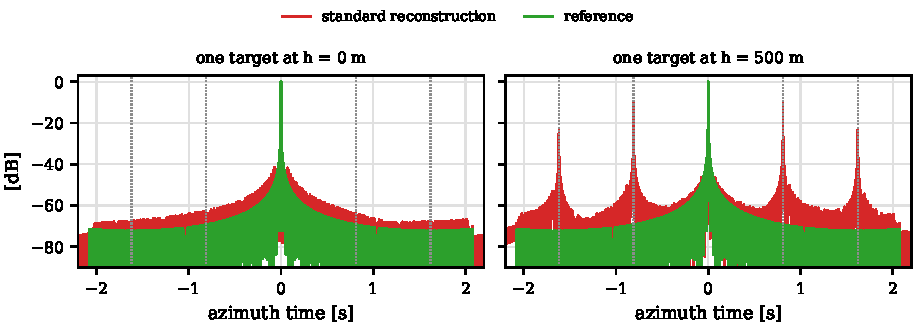
\includegraphics[width=\linewidth]{figures/irf_flat_vs_height.pdf}
\caption[Standard reconstruction of a target at the reference height and above it]{Impulse response of one target,
standard reconstruction and reference; dotted: ambiguity positions ($\pm1$, $\pm2$ times \SI{0.81}{s}). Left: $h=0$, the
responses coincide. Right: $h=\SI{500}{m}$.}
\label{fig:irfheight}
\end{figure}

\begin{figure}[htbp]
\centering
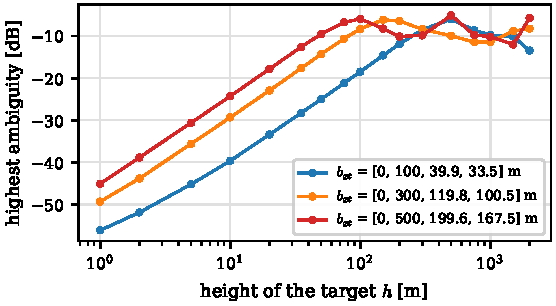
\includegraphics[width=0.62\linewidth]{figures/ambiguity_vs_height.pdf}
\caption[Highest ambiguity of the standard reconstruction against height]{Standard reconstruction, one target at height
$h$, three sets of baselines. At $h=0$ all give \SI{-63.6}{dB}, the band-limited reference level.}
\label{fig:ambheight}
\end{figure}

Since $c_m$ is the discrete Fourier transform of the channel phases, separating the parcels needs channels that see them with
\emph{different} phases: unequally spaced cross-track baselines and three or more channels.

\section{Ambiguity metric}\label{sec:metric}

The \emph{highest ambiguity} is the largest value of the impulse response, in dB relative to the reference peak, within
$\pm\SI{20}{ms}$ of the ambiguity positions ($\pm1$, $\pm2$ ambiguity distances) of every target. The reference (monostatic,
full rate, same band limit) sets the floor.
